%% IEEE Transactions on Mobile Computing version (IEEEtran, compsoc journal, two columns).
%% Single self-contained file. Proofs and additional results are in tmc_supp.tex (supplementary material).
\documentclass[10pt,journal,compsoc]{IEEEtran}

\usepackage[nocompress]{cite}
\usepackage{amsmath,amssymb,amsfonts}
\let\proof\relax
\let\endproof\relax
\usepackage{amsthm}
\usepackage{algorithm}
\usepackage{algpseudocode}
\usepackage{graphicx}
\usepackage{booktabs}
\usepackage{xcolor}
\usepackage{url}

\newtheorem{assumption}{Assumption}
\newtheorem{definition}{Definition}
\newtheorem{lemma}{Lemma}
\newtheorem{proposition}{Proposition}
\newtheorem{corollary}{Corollary}
\newtheorem{theorem}{Theorem}
\theoremstyle{remark}
\newtheorem{remark}{Remark}
\newtheorem{example}{Example}

\newcommand{\E}{\mathbb{E}}
\newcommand{\Prob}{\mathbb{P}}
\newcommand{\ind}[1]{\mathbf{1}\{#1\}}
\newcommand{\A}{\mathcal{A}}
\newcommand{\I}{\mathcal{I}}
\newcommand{\lab}{\ell}
\newcommand{\Dbar}{\bar{\Delta}}
\newcommand{\ee}{\varepsilon}
\newcommand{\xh}{\hat{x}}

\begin{document}

\title{Speak When Sure, Ask When Unsure: Confidence-Aware Status Updates from On-Board Classifiers in Aerial IoT}

\author{Sameh~Hosny%
\IEEEcompsocitemizethanks{\IEEEcompsocthanksitem S. Hosny is with the Electrical and Computer Engineering Department, American University of Armenia, Yerevan, Armenia.\protect\\
E-mail: sameh.hosny@aua.am}}

\markboth{IEEE Transactions on Mobile Computing}{Hosny: Confidence-Aware Status Updates from On-Board Classifiers in Aerial IoT}

\IEEEtitleabstractindextext{%
\begin{abstract}
On-board classifiers let Internet of Things (IoT) devices send a few-byte label instead of raw data, but a wrong label misleads the receiver. We study an unmanned aerial vehicle (UAV) that monitors a scene for a ground station (GS) and, in each slot, stays silent, sends its label, or uploads the frame to a more accurate ground classifier. It seeks a low average age of incorrect information (AoII) at the GS under an energy budget and an intermittent link. As the UAV never observes the true state, we formulate a constrained partially observable Markov decision process and show that a belief over the AoII, updated with each frame's calibrated confidence, is a sufficient statistic. We derive each action's one-step expected AoII in closed form, prove that a label that agrees with the GS is never worth sending, and show that drift-plus-penalty reduces to confidence thresholds ordered silent, raw, label. The policy, CA-DPP, meets the energy budget on every sample path. On Sentinel-2 flood-mapping traces, it lowers the AoII by 52 to 75 percent relative to pre-identification and age-threshold policies, and by up to 49 percent relative to an AoII-threshold policy when energy is scarce or the classifier is weak.
\end{abstract}

\begin{IEEEkeywords}
Age of incorrect information, on-board inference, confidence calibration, unmanned aerial vehicle, Internet of Things, Lyapunov optimization, POMDP.
\end{IEEEkeywords}}

\maketitle
\IEEEdisplaynontitleabstractindextext
\IEEEpeerreviewmaketitle

%% =====================================================================
%% =====================================================================
\IEEEraisesectionheading{\section{Introduction}\label{sec:intro}}
\IEEEPARstart{M}{any} Internet of Things (IoT) devices no longer send what they sense. A camera trap reports that it saw an animal, and an unmanned aerial vehicle (UAV) that surveys a flood reports that the area below it is under water. Each device runs a small classifier on board and transmits a label of a few bytes instead of an image of tens of kilobytes~\cite{shamsoshoara2021flame,kyrkou2020aider}, which saves most of the energy and airtime of a raw upload.

A classifier small enough to run on a UAV makes mistakes, mostly on ambiguous inputs such as a flooded field under cloud shadow or a dry field after rain. Once the transmitted content is an inference, a delivered update can be wrong, and the receiver keeps a fresh but wrong estimate until a later update corrects it. The age of information (AoI) misses this error, because it resets on every delivery. The age of incorrect information (AoII)~\cite{maatouk2020aoii} grows while the receiver's estimate differs from the true state, so it penalizes wrong estimates as well as stale ones.

Existing AoII work assumes that the transmitter observes the source through a sensor~\cite{maatouk2020aoii,zakeri2023aoiieh,ngo2025eh}, so it knows when the receiver is wrong. A device whose sensor is a classifier sees only its own label and how confident the classifier is about it. A confident label that disagrees with the receiver probably means that the receiver is wrong; an unsure label could mean either, and sending it may turn a correct estimate into a wrong one. The device can also upload the raw data and let a larger classifier on the ground decide, at a much higher energy cost that depends on the link.

Consider a UAV that maps a flood for a ground station (GS) that coordinates rescue teams. If a frame looks clearly flooded and the GS status says dry, the UAV should send its label. If the frame is ambiguous, it should upload the frame when the link is good enough, and wait otherwise. If its label agrees with the GS status, it should stay silent. This paper turns these rules of thumb into a policy with guarantees. Doing so is hard for four reasons: the UAV never observes whether the GS is wrong; the confidence of a small classifier is noisy, and its errors are correlated across overlapping frames; the delivery probability and energy of each action change as the UAV moves; and a fixed energy budget couples all decisions of the mission.

We address three questions. \emph{(Q1)} In each slot, should the UAV stay silent, send its label or upload the frame, given its label, confidence, link and energy? \emph{(Q2)} Does the per-frame confidence lower the AoII, and when? \emph{(Q3)} When is a raw upload worth its cost? We answer Q1 analytically and Q2 and Q3 on real inference traces. Our contributions are as follows.
\begin{enumerate}
\item \emph{Model.} We formulate confidence-aware status updating as a constrained partially observable Markov decision process (POMDP) that couples a calibrated per-sample error model of the on-board classifier, a ground classifier, an intermittent air-to-ground link and an energy budget. We show that a belief over the current AoII is a sufficient statistic and derive its update, with a prior correction and a tempered likelihood for errors that are correlated in time (Sections~\ref{sec:model} and~\ref{sec:problem}).
\item \emph{Structure.} We derive each action's one-step expected AoII in closed form, prove that a label that agrees with the GS has no value, and show that the per-slot decision has confidence thresholds: silent at low confidence, raw upload at intermediate confidence, label at high confidence (Section~\ref{sec:structure}).
\item \emph{Policy.} We build the online policy CA-DPP on these results and prove that it meets the energy budget on every sample path. It needs no knowledge of the confidence distribution, the blockage statistics or the trajectory, and its per-slot cost is linear in the size of the belief (Section~\ref{sec:lyap}).
\item \emph{Evaluation.} On inference traces from Sen1Floods11~\cite{bonafilia2020sen1floods11}, under chip-level cross-validation and against policies adapted from four recent designs~\cite{zakeri2023aoiieh,gan2025taoi,pehlivanoglu2026orbit,basnayaka2025aomi}, the per-frame confidence pays off under tight budgets and with weak classifiers, and raw uploads pay off near the GS at larger budgets. In a synthetic model that satisfies our assumptions, a full-information lower bound places CA-DPP within $14\%$ to $25\%$ of the optimum (Sections~\ref{sec:results} and~\ref{sec:discussion}).
\end{enumerate}

The rest of the paper is organized as follows. Section~\ref{sec:related} reviews related work, Sections~\ref{sec:model} to~\ref{sec:lyap} answer Q1, Section~\ref{sec:results} answers Q2 and Q3, Section~\ref{sec:discussion} discusses implications and limitations, and Section~\ref{sec:concl} concludes. The supplementary material contains the proofs, a worked example and additional results.
%% =====================================================================
\section{Related Work}\label{sec:related}
%% =====================================================================

\subsection{Age of Incorrect Information}
Maatouk et al.~\cite{maatouk2020aoii} introduced the AoII, which is zero while the receiver's estimate equals the source state and grows while the two differ. For a Markov source observed perfectly by the transmitter, the optimal policy transmits only when the estimate is wrong.

Zakeri et al.~\cite{zakeri2023aoiieh} study an energy-harvesting sensor that decides when to sample and transmit; since it does not see the source between samples, they formulate a POMDP with a belief about the source state and compute the AoII-optimal policy numerically, finding a multi-threshold structure. Ngo et al.~\cite{ngo2025eh} study the age and correctness of updates from many energy-harvesting devices on a random-access channel. In both works a sample reveals the source state without error. Our UAV never observes the state; it sees a classifier output that may be wrong, with an error probability that changes from frame to frame. Our belief is closest to that of Cosandal et al.~\cite{cosandal2024joint}, who keep a joint belief over the age and the source state at a monitor that pulls delayed samples. There a delivered sample is exact and the uncertainty comes from the delay; in our problem a fresh observation arrives in every slot but may be wrong, so the belief must weigh each frame by its confidence.


\subsection{Freshness of Inferred Information}
Buratto et al.~\cite{buratto2023misclass} add a misclassification penalty to an AoI scheduling problem with a fixed error probability and an offline schedule. Gan et al.~\cite{gan2025taoi} define a task-oriented AoI for cameras that pre-identify frames on the device and send those that appear to contain the target to a server for re-identification, with fixed error rates for both classifiers. Pehlivano\u{g}lu, Li and Uysal~\cite{pehlivanoglu2026orbit} let a satellite choose among idling, on-board inference, sending a cached result and offloading raw data, the action set closest to ours, and prove that a threshold policy minimizes the age of inference; each action succeeds with a fixed probability, errors do not depend on the sample, and energy is not constrained. Basnayaka et al.~\cite{basnayaka2025aomi} define the age of misclassified information for event detection from low Earth orbit with a constant accuracy. All these works describe the classifier by a single error rate. A calibrated classifier also reports, for each frame, how likely its label is to be wrong, and we use this in the decision.


\subsection{Inference Offloading from IoT Devices and UAVs}
Work on computation offloading decides whether an IoT device or a UAV should run a task locally or at an edge server, usually to minimize delay or energy; Yang et al.~\cite{yang2020uav}, for example, split a deep network for UAV target tracking between the UAV and an edge server. Such work does not measure how fresh or how correct the receiver's knowledge is. FLAME~\cite{shamsoshoara2021flame} and AIDER~\cite{kyrkou2020aider} show that classifiers small enough for a UAV reach useful accuracy but still err on a noticeable fraction of frames, and post-hoc calibration~\cite{guo2017calibration} makes their scores reliable probabilities. We handle the energy constraint with Lyapunov drift-plus-penalty~\cite{neely2010book}, which Huang and Neely~\cite{huang2013eh} extend to finite batteries; since the AoII depends on past decisions, the renewal framework of~\cite{neely2013renewal} is the natural tool for its performance analysis (Section~\ref{sec:lyap}).


Table~\ref{tab:positioning} compares the closest works on four elements: (E1) a per-sample error model driven by the confidence; (E2) AoII on the inferred label; (E3) an online energy constraint; and (E4) a choice among silence, a label and raw data. Each prior work covers at most two fully; ours combines all four.

\begin{table}[t]
\caption{Positioning against the closest works. \checkmark: covered; $\circ$: partly covered; --: not covered.}
\label{tab:positioning}
\centering\footnotesize
\setlength{\tabcolsep}{3pt}
\resizebox{\columnwidth}{!}{%
\begin{tabular}{@{}lcccc@{}}
\toprule
Work & (E1) per-sample & (E2) AoII on & (E3) online & (E4) silent/\\
 & errors & inferred label & energy & label/raw\\
\midrule
Zakeri et al.~\cite{zakeri2023aoiieh} & -- & \checkmark & $\circ$ & $\circ$\\
Ngo et al.~\cite{ngo2025eh} & -- & $\circ$ & $\circ$ & --\\
Buratto et al.~\cite{buratto2023misclass} & $\circ$ & \checkmark & -- & --\\
Gan et al.~\cite{gan2025taoi} & $\circ$ & $\circ$ & -- & $\circ$\\
Pehlivano\u{g}lu et al.~\cite{pehlivanoglu2026orbit} & -- & $\circ$ & -- & \checkmark\\
Basnayaka et al.~\cite{basnayaka2025aomi} & $\circ$ & $\circ$ & -- & --\\
Yang et al.~\cite{yang2020uav} & -- & -- & $\circ$ & $\circ$\\
\midrule
This work & \checkmark & \checkmark & \checkmark & \checkmark\\
\bottomrule
\end{tabular}}
\end{table}
%% =====================================================================
\section{System Model}\label{sec:model}
%% =====================================================================
\subsection{Network and Scenario}\label{sec:story}
A UAV flies over a disaster area and reports to a ground station (GS) that coordinates the response (Fig.~\ref{fig:system}). Time is slotted with slot length $\tau$ and index $t\in\{0,1,\dots\}$. The UAV flies at constant speed along a route planned before the mission, so its position $\mathbf{u}(t)$ is known in advance. In each slot it photographs the patch of ground below it, its footprint, and a small on-board classifier decides whether an event of interest, such as flooding, fire or a survivor, is present. We use flood mapping as the running example: each photo is labeled ``flooded'' or ``dry'', and the response teams need to know which patches are under water. The model applies to any such event with a suitable classifier.

Consecutive footprints partly overlap. We model only what the UAV sees along its route: $X(t)$ is the state of the patch below the UAV in slot $t$ and $Y(t)$ is its photo. The position enters only through the link, since the distance and elevation angle to the GS set the delivery probability and the energy of a packet. The route can have any shape; in our evaluation it is a circle, so the UAV alternately passes near the GS and far from it.

The GS has no sensor of its own. Its status for the current patch is the last label it received, either a label sent by the UAV or the label that a larger ground classifier produced from an uploaded photo, and the response teams act on it. In each slot the UAV can stay silent, send its label, or send the photo. A label is a few bytes and cheap but may be wrong; a photo is much more expensive and may fail far from the GS, but the ground classifier labels it almost always correctly. The UAV chooses under an energy budget and never observes the true state. Table~S1 in the supplementary material summarizes the notation.

\begin{figure}[t]
\centering
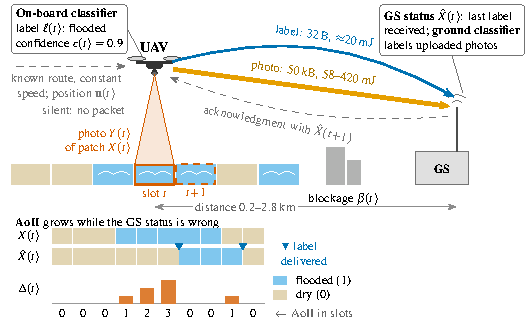
\includegraphics[width=0.8\columnwidth]{figures/fig_scenario.pdf}
\caption{System model. A UAV flies over a disaster area, photographs the patch below it and labels each photo on board with a confidence $c(t)$. In each slot it stays silent, sends its label (blue) or uploads the photo to the more accurate ground classifier (orange). The GS keeps the last label received and acks each decoded packet. Inset: the AoII grows while the GS status is wrong and resets when it becomes right. Values shown are examples from Section~\ref{sec:results}.}
\label{fig:system}
\end{figure}


\subsection{Event Dynamics}\label{sec:src}
The state $X(t)\in\{0,1\}$ is $1$ if the event is present (the patch is flooded) and $0$ otherwise. It refers to the patch below the UAV in slot $t$, not to a fixed patch. Because consecutive frames overlap, the state tends to persist, at a rate set by the speed of the UAV and the overlap of its footprints, both constant. We use the simplest model with this persistence, a two-state Markov chain (Fig.~S1 in the supplementary material). With $p_x$ the probability that the state leaves $x$ in one slot,
\begin{equation}\label{eq:source}
\Prob\big\{X(t+1)\neq x\mid X(t)=x\big\}=p_x,\qquad x\in\{0,1\}.
\end{equation}
We assume $0<p_0,p_1<\tfrac12$. The lower bound makes the chain irreducible; the upper bound says that the state is more likely to stay than to change, which is what makes an old status useful. Balancing the flows between the two states, $\varpi_0p_0=\varpi_1p_1$, gives the stationary distribution

\begin{equation}\label{eq:stationary}
\varpi_1=\frac{p_0}{p_0+p_1},\qquad \varpi_0=\frac{p_1}{p_0+p_1}.
\end{equation}
which we call the class prior. The chain may be asymmetric: a flooded footprint typically turns dry more often than a dry one floods ($p_1>p_0$), so $\varpi_1<\varpi_0$.

\subsection{On-Board and Ground Classification}
In slot $t$ the on-board classifier maps the photo $Y(t)$ to a label and a confidence,
\begin{equation}\label{eq:label}
\lab(t)\in\{0,1\},\qquad c(t)\in[\tfrac12,1],
\end{equation}
where $\lab(t)$ is the more likely state and $c(t)$ the probability the classifier assigns to it; a classifier that outputs a flood probability $p$ gives $\lab(t)=\ind{p\ge\frac12}$ and $c(t)=\max\{p,1-p\}$. We require calibration for each label value: among frames with label $\lab$ and confidence $c$, a fraction $c$ is truly in state $\lab$,
\begin{equation}\label{eq:calib}
\Prob\big\{X(t)=\lab(t)\mid\lab(t),\,c(t)\big\}=c(t).
\end{equation}
Hence a label with confidence $c$ is wrong with probability $1-c$. We need~\eqref{eq:calib} for each label value because flooded and dry patches are not equally common. Modern classifiers are often overconfident, but post-hoc calibration~\cite{guo2017calibration}, such as isotonic regression on held-out data, restores~\eqref{eq:calib} to a good approximation; Fig.~S2 in the supplementary material shows this for our models.


The belief update needs the likelihood of the pair $(\lab(t),c(t))$ under each state, but calibration gives the posterior. By~\eqref{eq:calib}, the posterior of state $x\in\{0,1\}$ is
\begin{equation}\label{eq:cx}
c_x(t)=\Prob\big\{X(t)=x\mid\lab(t),c(t)\big\}=\begin{cases}c(t), & x=\lab(t),\\ 1-c(t), & x\neq\lab(t).\end{cases}
\end{equation}
By Bayes' rule and~\eqref{eq:cx}, posterior and likelihood are related through the class prior,
\begin{equation}\label{eq:lik}
\Prob\big\{\lab(t),c(t)\mid X(t)=x\big\}=\frac{c_x(t)\,\Prob\big\{\lab(t),c(t)\big\}}{\varpi_x}\propto\frac{c_x(t)}{\varpi_x},
\end{equation}
since $\Prob\{\lab(t),c(t)\}$ does not depend on $x$. The division by $\varpi_x$ matters when classes are unbalanced: a frame with $c(t)=\frac12$ looks neutral, but it is $\varpi_0/\varpi_1$ times more likely under $X=1$ than under $X=0$. The classifier has already used the prior, and the belief update uses the source dynamics, which contain it again; dividing by $\varpi_x$ avoids counting it twice.

After a raw upload, the ground classifier returns a label $\lab^{\rm g}(t)$. It is larger and sees all spectral bands, so it is more accurate, but frames that are hard on board are often hard on the ground as well. We therefore let its error probability depend on the on-board confidence and write $\ee_{\rm g}(c)$. The following assumption is used only to design the controller; the simulations replay real classifier outputs, which do not satisfy it exactly.



\begin{assumption}[Inference model]\label{as:inf}
(i) The on-board classifier is calibrated, i.e.,~\eqref{eq:calib} holds. (ii) Given the source path, the on-board outputs $(\lab(t),c(t))$ are independent across slots. (iii) Given $X(t)$ and $c(t)=c$, the ground label is wrong with probability $\ee_{\rm g}(c)<\tfrac12$, independently of $\lab(t)$ and of the past.
\end{assumption}

Part (ii) is the strongest. Overlapping footprints make errors come in runs (Section~\ref{res:cls}). We keep (ii) because it gives a tractable belief update and correct for its optimism in Section~\ref{sec:update}.

\subsection{Actions and Channel}\label{sec:act}
After classifying the frame, the UAV chooses $a(t)\in\A=\{0,1,2\}$. It stays silent ($a=0$), which costs nothing; sends its label in a packet of $L_1$ bits ($a=1$), which corrects a wrong GS status if the label is right and spoils a correct one if it is wrong; or uploads the frame in $L_2\gg L_1$ bits ($a=2$) for the ground classifier.

Delivery depends on the link state $g(t)=(\mathbf{u}(t),\beta(t))$, the known position and a blockage indicator $\beta(t)\in\{0,1\}$. Buildings and terrain block the link for several slots at a time, so $\beta(t)$ is a two-state Markov chain with
\begin{equation}\label{eq:block}
\begin{split}
\Prob\big\{\beta(t+1)=1\mid\beta(t)=0\big\}&=\rho_{\rm b},\\
\Prob\big\{\beta(t+1)=0\mid\beta(t)=1\big\}&=\rho_{\rm u}.
\end{split}
\end{equation}
A blockage lasts $1/\rho_{\rm u}$ slots on average, a fraction $\rho_{\rm b}/(\rho_{\rm b}+\rho_{\rm u})$ of slots is blocked, and no packet gets through a blocked link. Otherwise the link is in line of sight (LoS) with a probability that grows with the elevation angle $\phi$, and following~\cite{alhourani2014lap} the mean path loss at distance $r$ is

\begin{equation}\label{eq:pl}
\overline{\rm PL}(r,\phi)={\rm FSPL}(r)+P_{\rm LoS}(\phi)\,\eta_{\rm LoS}+\big(1-P_{\rm LoS}(\phi)\big)\eta_{\rm NLoS},
\end{equation}
where ${\rm FSPL}(r)$ is the free-space path loss, $\eta_{\rm LoS}$ and $\eta_{\rm NLoS}$ are excess losses, and $P_{\rm LoS}(\phi)=[1+\alpha e^{-b(\phi-\alpha)}]^{-1}$ with environment constants $\alpha$, $b$. With the transmit power, bandwidth $W$ and noise figure, \eqref{eq:pl} gives the mean signal-to-noise ratio (SNR) $\bar\gamma(g)$.

Under Rayleigh block fading the instantaneous SNR is $\bar\gamma(g)|h|^2$ with $|h|^2$ exponential of unit mean. The UAV sends $L_a$ bits with a rateless code until the GS decodes and acknowledges the packet or a window $\tau_{\max}\le\tau$ ends, so the packet is decoded if $W\tau_{\max}\log_2(1+\bar\gamma|h|^2)\ge L_a$, with probability
\begin{equation}\label{eq:succ}
q_a(g)=(1-\beta)\,\exp\!\Big(-\frac{\gamma_a}{\bar\gamma(g)}\Big),\qquad \gamma_a=2^{L_a/(W\tau_{\max})}-1,
\end{equation}
for $a\in\{1,2\}$,
and $q_0\equiv0$, where $\gamma_a$ is the SNR needed to deliver $L_a$ bits in the window; $L_2>L_1$ gives $q_2(g)\le q_1(g)$.

The link is an erasure channel. Every packet carries an $n$-bit cyclic redundancy check (CRC), so a corrupted packet passes with probability about $2^{-n}$, and the GS acknowledges only decoded packets; a missing acknowledgment tells the UAV that the GS status did not change. Acknowledgments are short and sent at higher power, so we assume they always arrive. Remark~S1 in the supplementary material shows that undetected bit errors in a label can cancel an update but never make a correct GS status wrong.


\subsection{Energy Consumption}
A transmission costs the radio energy while it transmits, $P_{\rm r}\E_h[\min\{L_a/C(h),\tau_{\max}\}]$ with $C(h)=W\log_2(1+\bar\gamma|h|^2)$, plus a per-packet overhead $E_{\rm o}$ for wake-up, channel access and the acknowledgment. The controller needs this value before $h$ is known, so we evaluate the airtime at the mean rate $\bar R(g)=W\log_2(1+\bar\gamma(g))$:
\begin{equation}\label{eq:energy}
E_a(g)=P_{\rm r}\min\Big\{\frac{L_a}{\bar R(g)},\tau_{\max}\Big\}+E_{\rm o},\quad a\in\{1,2\},
\end{equation}
and $E_0=0$. For a label the overhead dominates and the approximation is accurate; for a raw frame it is least accurate at intermediate distances, and Section~\ref{sec:results} quantifies the gap. Capture, inference and propulsion~\cite{zeng2019rotary} cost the same for every decision, so we constrain only the communication energy, through a long-run average budget of $\bar E$ joules per slot:
\begin{equation}\label{eq:budget}
\limsup_{T\to\infty}\frac1T\sum_{t=0}^{T-1}\E\Big[E_{a(t)}\big(g(t)\big)\Big]\le\bar E.
\end{equation}
The $\limsup$ is needed because the running average need not converge for every policy. An average budget lets the UAV spend more where uploads are cheap, near the GS, and less elsewhere.

\subsection{The GS Status and the AoII}
Let $o(t)\in\{0,1\}$ indicate that the packet of slot $t$ is decoded, with $\Prob\{o(t)=1\mid a(t)=a,g(t)=g\}=q_a(g)$. The GS status $\hat X(t)$ is the most recent label received:
\begin{equation}\label{eq:est}
\hat X(t+1)=\begin{cases}\lab(t), & a(t)=1,\ o(t)=1,\\ \lab^{\rm g}(t), & a(t)=2,\ o(t)=1,\\ \hat X(t), & \text{otherwise.}\end{cases}
\end{equation}
Holding the last label is the natural estimator for a persistent state. Each acknowledgment carries $\hat X(t+1)$, so the UAV always knows $\hat X(t)$, but never $X(t)$.

The GS status becomes wrong when the scene changes before the UAV reports it, or when a wrong label reaches the GS and spoils a correct status. A status wrong for one slot does little harm; one wrong for a minute may send a team to the wrong place. We therefore use the AoII~\cite{maatouk2020aoii}, which is zero while the status is correct and otherwise counts the slots for which it has been wrong:
\begin{equation}\label{eq:aoii}
\Delta(t+1)=\big(\Delta(t)+1\big)\,\ind{X(t+1)\neq\hat X(t+1)},\quad \Delta(0)=0.
\end{equation}
Unlike the AoI, the AoII grows right after a wrong delivery, and it penalizes long errors more than fresh ones. Table~S2 in the supplementary material traces it through a short example.




\subsection{Order of Events}\label{sec:events}
Within slot $t$, the UAV observes $g(t)$, captures $Y(t)$ and computes $\lab(t)$, $c(t)$; it chooses $a(t)$ and transmits if $a(t)\neq0$; the packet is decoded with probability $q_{a(t)}(g(t))$, in which case the GS updates its status by~\eqref{eq:est} and acknowledges; finally the scene moves to $X(t+1)$ and the AoII to $\Delta(t+1)$ by~\eqref{eq:aoii}.
%% =====================================================================
\section{Problem Formulation}\label{sec:problem}
%% =====================================================================

\subsection{Information and Policies}
When it chooses $a(t)$, the UAV knows its labels, confidences and link states up to slot $t$ and the outcome of every earlier transmission,
\begin{equation}\label{eq:info}
\I(t)=\big\{\lab(s),c(s),g(s)\big\}_{s\le t}\cup\big\{a(s),\hat X(s+1)\big\}_{s<t},
\end{equation}
together with the ground label of every decoded upload.
but not $X(t)$, so it cannot compute $\Delta(t)$. A policy $\psi$ maps $\I(t)$ to a distribution on $\A$; randomization may be needed to use an average budget exactly. Transmitting on a blocked link is pointless, so $\Psi$ denotes the policies with $a(t)=0$ whenever $q_1(g(t))=0$.

\subsection{The Optimization Problem}
The long-run average AoII grows both with the fraction of slots in which the GS is wrong and with the length of the wrong periods. Under a policy $\psi$, the average AoII and energy are
\begin{align}
\bar\Delta^{\psi}&=\limsup_{T\to\infty}\frac1T\sum_{t=0}^{T-1}\E^{\psi}\big[\Delta(t)\big],\label{eq:avgaoii}\\
\bar E^{\psi}&=\limsup_{T\to\infty}\frac1T\sum_{t=0}^{T-1}\E^{\psi}\Big[E_{a(t)}\big(g(t)\big)\Big],\label{eq:avgE}
\end{align}
where $\E^{\psi}$ is the expectation under $\psi$. The UAV solves
\begin{equation}\label{eq:P}
\textbf{(P)}\qquad \min_{\psi\in\Psi}\ \bar\Delta^{\psi}\qquad\text{subject to}\qquad \bar E^{\psi}\le\bar E.
\end{equation}

Problem (P) is hard for three reasons: the cost depends on $X(t)$, which the UAV never sees; the cost has memory, since a wrong status adds to the AoII in every slot until it is corrected; and the budget couples all slots. We handle the first exactly below, by replacing the unknown AoII with a distribution over its values. Section~\ref{sec:structure} handles the second by valuing each action through its effect on the next slot, and Section~\ref{sec:lyap} handles the third by pricing energy by what has been spent.

\subsection{A Belief on the AoII}\label{sec:belief}
The information $\I(t)$ grows with $t$, but a much smaller object suffices.

\begin{lemma}[Sufficient statistic]\label{lem:suff}
Given $\hat X(t)$, the AoII determines the state: $X(t)=\hat X(t)$ if $\Delta(t)=0$ and $X(t)=1-\hat X(t)$ if $\Delta(t)>0$. Hence the pair $(\hat X(t),\pi_t)$, together with the link state $g(t)$ that the UAV observes, where
\begin{equation}\label{eq:belief}
\pi_t(\delta)=\Prob\big\{\Delta(t)=\delta\mid\I(t)\big\},\qquad\delta\in\{0,1,\dots\},
\end{equation}
summarizes $\I(t)$ for predicting the future AoII.
\end{lemma}
\begin{proof}
By~\eqref{eq:aoii}, $\Delta(t)>0$ iff $X(t)\neq\hat X(t)$, so $(\hat X(t),\Delta(t))$ determines the binary $X(t)$. By~\eqref{eq:source} and Assumption~\ref{as:inf}, the future scene and classifier outputs then depend on $\I(t)$ only through $\hat X(t)$ and $\pi_t$; the link evolves independently of the scene, and its current state $g(t)$ is observed.
\end{proof}

The mass of $\pi_t$ at $0$ is the probability that the GS is correct. For each $\delta$ we write $x_\delta$ for the state implied by Lemma~\ref{lem:suff}: $x_0=\hat X(t)$ and $x_\delta=1-\hat X(t)$ for $\delta>0$. To store the belief we truncate its support at $\Delta_{\max}$, adding the mass above it to $\pi_t(\Delta_{\max})$; this is harmless when $\Delta_{\max}$ is well above the AoII values that occur, which Section~\ref{sec:results} checks.


\subsection{Belief Update}\label{sec:update}
Let $\pi^-_t$ be the belief at the start of slot $t$, before the new frame is classified. The update has three steps.

\emph{Step 1: on-board label.} By Bayes' rule,
\begin{equation}\label{eq:bayes}
\pi_t(\delta)\propto\pi^-_t(\delta)\,\Prob\big\{\lab(t),c(t)\mid\Delta(t)=\delta,\I(t-1)\big\}.
\end{equation}
Under Assumption~\ref{as:inf}(ii), the frame depends on the past only through the current state $x_\delta$, so by~\eqref{eq:lik} the likelihood is proportional to $c_{x_\delta}(t)/\varpi_{x_\delta}$. All $\delta>0$ imply the same state, so only the ratio between ``GS wrong'' and ``GS right'' matters. With $d(t)=\ind{\lab(t)\neq\hat X(t)}$ indicating that the label disagrees with the GS, this ratio is
\begin{equation}\label{eq:Lambda}
\Lambda_t=\frac{c_{1-\hat X(t)}(t)}{c_{\hat X(t)}(t)}\cdot\frac{\varpi_{\hat X(t)}}{\varpi_{1-\hat X(t)}},
\end{equation}
By~\eqref{eq:cx}, the first factor is $c(t)/(1-c(t))$ if $d(t)=1$ and $(1-c(t))/c(t)$ if $d(t)=0$. A disagreeing label is thus evidence that the GS is wrong, more so the more confident it is, and an agreeing label is evidence that the GS is right.

Exact Bayes' rule multiplies the odds that the GS is wrong by $\Lambda_t$. This treats every frame as independent and overstates the evidence when errors come in runs: a second miss of the same flood in an overlapping frame is not independent confirmation. We therefore temper the ratio with an exponent $\nu\in(0,1]$, a practical correction chosen on data. With $\mu^-_t=\pi^-_t(\Delta>0)$,
\begin{equation}\label{eq:post}
\pi_t(\delta)=\frac{\pi^-_t(\delta)}{1-\mu^-_t+\mu^-_t\Lambda_t^{\nu}}\times\begin{cases}1, & \delta=0,\\ \Lambda_t^{\nu}, & \delta>0.\end{cases}
\end{equation}
Each frame then counts as a fraction $\nu$ of an independent observation, and $\nu=1$ is Bayes' rule. A rough guide is the inverse of the mean length of an error run. More precisely, if the error indicators of consecutive frames have lag-$k$ correlation $\kappa^k$, $n$ frames carry roughly the evidence of $n(1-\kappa)/(1+\kappa)$ independent ones, which suggests $\nu=(1-\kappa)/(1+\kappa)$. In the evaluation we select $\nu$ on tuning data; Section~S3.5 of the supplementary material reports results with this correlation rule instead. We also allow the symmetric update that uses $\varpi_0=\varpi_1$ and $\nu=1$. Step~1 moves mass between $\delta=0$ and $\delta>0$ but keeps the shape of the belief within $\delta>0$.


\emph{Step 2: ground label.} After a decoded upload, \eqref{eq:post} is applied again with $\nu=1$ and ratio $(1-\ee_{\rm g})/\ee_{\rm g}$ if the ground label disagrees with $\hat X(t)$ and $\ee_{\rm g}/(1-\ee_{\rm g})$ otherwise, where $\ee_{\rm g}=\ee_{\rm g}(c(t))$; no prior correction is needed since $\ee_{\rm g}$ is defined given the state.

\emph{Step 3: prediction.} After the transmission the GS holds $\xh'=\hat X(t+1)$, known to the UAV. Under hypothesis $\delta$ the state $x_\delta$ is known, and by~\eqref{eq:aoii} the AoII grows to $\delta+1$ if $X(t+1)\neq\xh'$ and resets otherwise:
\begin{equation}\label{eq:pred}
\Prob\big\{\Delta(t+1)=\delta+1\mid\Delta(t)=\delta\big\}=\begin{cases}p_{x_\delta}, & x_\delta=\xh',\\ 1-p_{x_\delta}, & x_\delta\neq\xh',\end{cases}
\end{equation}
with $\Delta(t+1)=0$ otherwise. Summing over $\delta$ gives $\pi^-_{t+1}$. A delivered label that flips the status swaps the two cases, which moves the mass back towards $\delta=0$. We use two summaries,

\begin{equation}\label{eq:musum}
\mu_t=\pi_t(\Delta>0),\qquad S_t=\E_{\pi_t}\big[(\Delta+1)\ind{\Delta>0}\big].
\end{equation}
the probability that the GS is wrong and the AoII each wrong hypothesis will have in the next slot if the GS stays wrong; $\mu^-_t$ and $S^-_t$ are the same summaries of $\pi^-_t$.


\begin{example}\label{ex:belief}
Let the GS report ``not flooded'' ($\hat X(t)=0$), and let the UAV hold the belief $\pi^-_t(0)=0.95$, $\pi^-_t(1)=0.05$: it is fairly sure the GS is right. A frame then arrives with label ``flooded'' and confidence $c=0.9$, so $d(t)=1$. With $\varpi_0=0.81$ and $\varpi_1=0.19$,~\eqref{eq:Lambda} gives $\Lambda_t=(0.81/0.19)(0.9/0.1)=38.4$: the frame is $38$ times more likely if the GS is wrong. With exact Bayes' rule ($\nu=1$),~\eqref{eq:post} gives $\mu_t=0.05\cdot38.4/(0.95+0.05\cdot38.4)=0.67$: one confident frame makes the GS more likely wrong than right. With $\nu=0.5$ the same frame gives only $\mu_t=0.25$, and with $\nu=0.25$ it gives $\mu_t=0.12$. Suppose the UAV stays silent. The prediction~\eqref{eq:pred} with $p_0=0.039$ and $p_1=0.166$ gives $\mu^-_{t+1}=0.23$ for $\nu=0.5$. If the next frame again says ``flooded'' with $c=0.9$, the belief rises to $\mu_{t+1}=0.65$. With the tempered update, the UAV therefore needs two consistent frames to become as convinced as one frame makes it under exact Bayes' rule. Section~\ref{sec:structure} continues this example to show what the UAV does in each of these two slots.
\end{example}

By Lemma~\ref{lem:suff}, (P) is a constrained Markov decision process on $(\pi^-_t,\hat X(t),\lab(t),c(t),g(t))$ with per-slot cost $\E[\Delta(t+1)\mid\I(t),a(t)]$. Solving it by value iteration with a Lagrange multiplier is impractical on a UAV: the belief lives in a high-dimensional simplex, and the kernel and the right multiplier depend on the confidence law, the blockage and the trajectory, which change between missions. We instead value each action in closed form (Section~\ref{sec:structure}) and price energy online (Section~\ref{sec:lyap}).

%% =====================================================================
\section{The Value of Each Action}\label{sec:structure}
%% =====================================================================
A policy must weigh, in each slot, how much each action lowers the AoII against its energy. We value an action by its effect on the next slot, which depends only on the current belief, and leave later effects to the energy price. Fix slot $t$, let $\xh=\hat X(t)$, and write
\begin{equation}\label{eq:rw}
r=p_{\xh},\qquad w=p_{1-\xh}.
\end{equation}
the probabilities that the state leaves the value the GS reports and the other value; both are below $\frac12$.

\subsection{One-Step Expected AoII}
For hypothesis $\delta$ and new status $\xh'$, $\Delta(t+1)$ is $\delta+1$ or $0$, so its mean is $(\delta+1)$ times the probability in~\eqref{eq:pred}. The actions differ only in the status they produce. Assuming delivery and averaging over $\pi_t$:

\emph{Silence} keeps $\xh'=\xh$. For $\delta=0$ the probability is $r$; for $\delta>0$ it is $1-w$, so
\begin{equation}\label{eq:J0}
J_0=(1-\mu_t)\,r+S_t\,(1-w).
\end{equation}

\emph{Label.} If $d(t)=0$ nothing changes and the result is $J_0$. If $d(t)=1$ the status flips, the case $\delta=0$ has probability $1-r$ and $\delta>0$ has $w$, so
\begin{equation}\label{eq:J1}
J_1=(1-\mu_t)(1-r)+S_t\,w.
\end{equation}

\emph{Raw upload.} The ground label equals $X(t)$ with probability $1-\ee_{\rm g}$, independently of $\Delta(t)$ given $c(t)$ (Assumption~\ref{as:inf}(iii)). A correct ground label gives probability $p_{x_\delta}$ ($r$ or $w$), a wrong one $1-p_{x_\delta}$, so
\begin{equation}\label{eq:J2}
J_2=(1-\mu_t)\big[r+\ee_{\rm g}(1-2r)\big]+S_t\big[w+\ee_{\rm g}(1-2w)\big].
\end{equation}

A packet is delivered with probability $q_a(g)$ independently of the scene given $g$, so the expected AoII after action $a$ is $J_0-q_a(J_0-J_a)$. We call $G_a=J_0-J_a$ the gain of action $a$.

\begin{lemma}[One-step expected AoII]\label{lem:onestep}
Under Assumption~\ref{as:inf}, $\E[\Delta(t+1)\mid\I(t),a(t)=a]=J_0-q_a(g)\,G_a$, with $G_0=0$ and
\begin{align}
G_1&=\big[S_t(1-2w)-(1-\mu_t)(1-2r)\big]\,d(t), \label{eq:G1}\\
G_2&=(1-\ee_{\rm g})\,S_t(1-2w)-\ee_{\rm g}\,(1-\mu_t)(1-2r). \label{eq:G2}
\end{align}
\end{lemma}

The lemma is exact when $\pi_t$ is the posterior ($\nu=1$, no truncation); with $\nu<1$ the controller evaluates it at the tempered belief, and the structural results below hold for any $\nu\in(0,1]$.

Both gains combine two nonnegative terms. The term $S_t(1-2w)$ is the AoII an update removes when the GS is wrong and the update is right, and the term $(1-\mu_t)(1-2r)$ is the AoII it creates when the GS is right and the update is wrong. A disagreeing label removes the first in full, since it must be right if the GS is wrong, and creates the second in full. A ground label removes the first with probability $1-\ee_{\rm g}$ and creates the second only with probability $\ee_{\rm g}$. The label is a bold update and the upload a cautious one: a probably wrong label has $G_1<0$, while $G_2>0$ as soon as $S_t(1-2w)(1-\ee_{\rm g})>\ee_{\rm g}(1-\mu_t)(1-2r)$, which holds for a small probability of a wrong GS when the ground classifier is accurate.


\setcounter{example}{0}
\begin{example}[continued]
In slot $t$ of Example~\ref{ex:belief} with $\nu=0.5$, the belief is $\mu_t=0.25$ and $S_t=0.49$, and the ground error at $c=0.9$ is $\ee_{\rm g}=0.028$ (Fig.~S2(b) in the supplementary material). With $\xh=0$, $r=p_0=0.039$ and $w=p_1=0.166$. Lemma~\ref{lem:onestep} gives $G_1=-0.37$ and $G_2=0.30$: sending the label would more likely harm than help, while asking the ground would help. In slot $t+1$, after the second disagreeing frame, $\mu_{t+1}=0.65$ and the gains become $G_1=0.94$ and $G_2=1.21$. Now the GS is probably wrong, and the label is worth sending.
\end{example}

For a symmetric source the gains depend on the mean of the belief.

\begin{corollary}[Symmetric source]\label{cor:sym}
If $p_0=p_1=p$, then with $\Dbar_t=\E_{\pi_t}[\Delta(t)]$,
\begin{align*}
G_1&=(1-2p)\big(\Dbar_t+2\mu_t-1\big)\,d(t),\\
G_2&=(1-2p)\big(\mu_t+(1-\ee_{\rm g})\Dbar_t-\ee_{\rm g}\big).
\end{align*}
\end{corollary}
\begin{proof}
With $r=w=p$, both terms of the gains carry the factor $1-2p$. Since $S_t=\E_{\pi_t}[\Delta\ind{\Delta>0}]+\mu_t=\Dbar_t+\mu_t$, substituting in~\eqref{eq:G1} and~\eqref{eq:G2} gives the result.
\end{proof}

A disagreeing label thus lowers the expected AoII if and only if $\Dbar_t+2\mu_t>1$. When the GS has just become wrong, $\Dbar_t\approx\mu_t$ and the test is $\mu_t>\frac13$; as it stays wrong, a smaller $\mu_t$ suffices. The test does not depend on $p$.

\subsection{Agreeing Labels}

\begin{proposition}[No confirmations]\label{prop:confirm}
If $d(t)=0$, then $G_1=0$. Hence a policy that minimizes the expected AoII plus a nonnegative energy price never needs to send a label that agrees with the GS.
\end{proposition}
\begin{proof}
If $d(t)=0$, a delivered label leaves the status unchanged, so $J_1=J_0$ and $G_1=0$. Sending it then costs $E_1(g)>0$ and changes nothing else, so silence does at least as well for any energy price $\lambda\ge0$.
\end{proof}

This rules out designs in which the device reports every label so that the receiver can confirm its status; the pre-identification baseline of Section~\ref{sec:results} spends most of its energy on such labels.

\subsection{Threshold Structure of the Per-Slot Decision}
A per-slot rule must convert AoII into energy. We consider
\begin{equation}\label{eq:rule}
a(t)\in\arg\max_{a\in\A}\big\{V\,q_a(g)\,G_a-\lambda(t)\,E_a(g)\big\},
\end{equation}
where $V>0$ weighs the AoII and $\lambda(t)\ge0$ is a price per joule; Section~\ref{sec:lyap} shows that drift-plus-penalty yields this rule with $\lambda(t)$ equal to an energy debt. The confidence enters the gains only through $\Lambda_t$, which increases in $c$ if $d(t)=1$ and decreases if $d(t)=0$.


\begin{lemma}[Monotonicity in the evidence]\label{lem:mono}
Fix $\pi^-_t$. For any $A,B\ge0$, the quantity $AS_t-B(1-\mu_t)$ is a nondecreasing function of $\Lambda_t$.
\end{lemma}

The proofs of Lemma~\ref{lem:mono}, Proposition~\ref{prop:threshold} and Theorem~\ref{thm:budget} are in Section~S2 of the supplementary material.

\begin{proposition}[Confidence thresholds]\label{prop:threshold}
Fix $\pi^-_t$, $\hat X(t)$, $g$ and $\lambda(t)$, and let $I$ be an interval of confidences on which $\ee_{\rm g}(c)$ is constant, such as one bin of the estimate used in Section~\ref{sec:results}. For $c\in I$:
\begin{enumerate}
\item[(a)] If $d(t)=1$, there are thresholds $c_{\rm r}\le c_{\lab}$ such that~\eqref{eq:rule} stays silent for $c<c_{\rm r}$, uploads the frame for $c_{\rm r}\le c<c_{\lab}$, and sends the label for $c\ge c_{\lab}$. Any of the three intervals may be empty.
\item[(b)] If $d(t)=0$, it uploads the frame if and only if $c\le c^0_{\rm r}$ for some threshold $c^0_{\rm r}$, and stays silent otherwise.
\item[(c)] For fixed $\mu^-_t$, the silent regions shrink as $S^-_t$ grows, and they grow with $\lambda(t)$.
\end{enumerate}
\end{proposition}

Across bins the thresholds can shift where $\ee_{\rm g}(c)$ jumps. Part (a) is the rule of the title: a disagreeing frame is sent as a label when the UAV is sure, sent to the ground when it is unsure, and withheld when it is too unsure for either to pay off. By part (b), an unsure agreeing frame can still be worth uploading, since it leaves room for the GS to be wrong. By part (c), the UAV acts more readily the longer the GS has probably been wrong and less readily as energy becomes costlier.


\setcounter{example}{0}
\begin{example}[continued]
Let the UAV be $1.2$\,km from the GS, where $q_1\approx1$, $q_2=0.78$, $E_1=20$\,mJ and $E_2=190$\,mJ. In slot $t$, the label has $q_1G_1<0$, and the upload has $q_2G_2=0.23$, so~\eqref{eq:rule} uploads the frame if $\lambda/V<0.23/0.19=1.2$\,J$^{-1}$ and stays silent otherwise. In slot $t+1$, $q_1G_1=0.94$ and $q_2G_2=0.95$ are almost equal, but the label costs a tenth of the upload, so the UAV sends the label for any price between about $0.05$ and $47$\,J$^{-1}$. At the price $\lambda/V=2$\,J$^{-1}$ used in Fig.~\ref{fig:regions}, the UAV thus waits in slot $t$ and sends the label in slot $t+1$.
\end{example}

\begin{figure}[t]
\centering
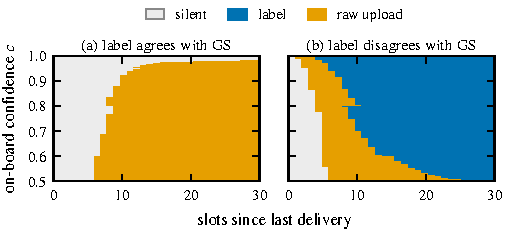
\includegraphics[width=0.8\columnwidth]{figures/regions.pdf}
\caption{Example of the decisions of~\eqref{eq:rule} versus the slots since the last delivery and the on-board confidence $c$. The GS reports ``not flooded'' with $5\%$ initial doubt, the UAV is $1.2$\,km from the GS ($q_1\approx1$, $q_2=0.78$, $E_1=20$\,mJ, $E_2=190$\,mJ), $\lambda/V=2$\,J$^{-1}$ and $\nu=0.25$. (a) An agreeing label is never sent; the frame is uploaded once the status is old, unless the UAV is very confident. (b) A disagreeing frame is uploaded when the UAV is unsure and sent as a label when it is confident (Proposition~\ref{prop:threshold}). Steps come from the binned estimate of $\ee_{\rm g}(c)$.}
\label{fig:regions}
\end{figure}

Fig.~\ref{fig:regions} shows the regions of~\eqref{eq:rule} for the setting of Example~\ref{ex:belief}, with the binned $\ee_{\rm g}(c)$ estimated from our data; the order silent, raw, label holds. The confidence needed to send a disagreeing label falls as the status ages, and an unsure agreeing frame is uploaded once the status is old enough, which asks the GS to verify its status.
%% =====================================================================
\section{Online Policy: CA-DPP}\label{sec:lyap}
%% =====================================================================
A fixed price in~\eqref{eq:rule} would have to be tuned to the mission. We derive the price from the energy spent with drift-plus-penalty~\cite{neely2010book}.

\subsection{Energy Debt as a Virtual Queue}
The energy debt evolves as the virtual queue
\begin{equation}\label{eq:Z}
Z(t+1)=\max\Big\{Z(t)+E_{a(t)}\big(g(t)\big)-\bar E,\ 0\Big\},\qquad Z(0)=0.
\end{equation}
Since $\max\{z,0\}\ge z$, summing over $t<T$ gives
\begin{equation}\label{eq:Zbound}
\frac1T\sum_{t=0}^{T-1}E_{a(t)}\big(g(t)\big)\le\bar E+\frac{Z(T)}{T},
\end{equation}
so the budget holds whenever the debt grows sublinearly.

\subsection{Drift-Plus-Penalty}
With $L(t)=\frac12Z(t)^2$, squaring~\eqref{eq:Z} and using $\max\{z,0\}^2\le z^2$,
\[
Z(t+1)^2\le Z(t)^2+\big(E_{a(t)}-\bar E\big)^2+2Z(t)\big(E_{a(t)}-\bar E\big).
\]
The middle term is at most $\max\{E_{\max},\bar E\}^2$ with $E_{\max}=\max_{a,g}E_a(g)$, so
\begin{equation}\label{eq:drift}
\E\big[L(t+1)-L(t)\,|\,\I(t)\big]\le C+Z(t)\,\E\Big[E_{a(t)}\big(g(t)\big)-\bar E\,\big|\,\I(t)\Big],
\end{equation}
with $C=\frac12\max\{E_{\max},\bar E\}^2$. Minimizing the right side plus $V$ times the expected next-slot AoII gives, by Lemma~\ref{lem:onestep},
\[
\min_{a\in\A}\Big\{Z(t)E_a(g)+V\big(J_0-q_a(g)G_a\big)\Big\}.
\]
Dropping the terms that do not depend on the action gives~\eqref{eq:rule} with $\lambda(t)=Z(t)$: the energy price is the energy debt. Overspending enlarges the silent regions of Proposition~\ref{prop:threshold}(c); underspending drains the debt to zero, and every useful update is sent. Algorithm~\ref{alg:dpp} lists the resulting confidence-aware drift-plus-penalty (CA-DPP) policy.


\begin{algorithm}[t]
\caption{CA-DPP, executed by the UAV in slot $t$}\label{alg:dpp}
\begin{algorithmic}[1]
\State Classify $Y(t)$ to get $\lab(t)$, $c(t)$; observe $g(t)$; set $d(t)$
\State Correct $\pi^-_t\to\pi_t$ by~\eqref{eq:post}; compute $\mu_t$, $S_t$
\State Compute $G_1$, $G_2$ by~\eqref{eq:G1}--\eqref{eq:G2}
\If{$q_1(g(t))=0$} $a(t)\gets0$
\Else\ $a(t)\gets\arg\max_a\{Vq_a(g)G_a-Z(t)E_a(g)\}$, ties to silence, then to upload
\EndIf
\State Transmit; read the acknowledgment: $\hat X(t+1)$, and $\lab^{\rm g}(t)$ after a decoded raw upload
\State If a ground label arrived, correct $\pi_t$ with it (Step 2)
\State Predict $\pi^-_{t+1}$ by~\eqref{eq:pred}
\State $Z(t+1)\gets\max\big\{Z(t)+E_{a(t)}(g(t))-\bar E,0\big\}$
\end{algorithmic}
\end{algorithm}


\subsection{Energy Guarantee}
\begin{theorem}[Budget]\label{thm:budget}
Let $E_{\min}=\min_{a\neq0,g}E_a(g)>0$. Under CA-DPP, for every sample path and every $t$,
\begin{equation}\label{eq:Zmax}
Z(t)\le Z_{\max}=\frac{V(\Delta_{\max}+1)}{E_{\min}}+E_{\max}.
\end{equation}
Consequently, $\frac1T\sum_{t<T}E_{a(t)}(g(t))\le\bar E+Z_{\max}/T$ for every $T$, and~\eqref{eq:budget} holds.
\end{theorem}

A gain never exceeds $\Delta_{\max}+1$, so once $Z(t)E_a(g)>V(\Delta_{\max}+1)$ for every transmission the UAV stays silent and the debt drains. The bound is loose; Section~\ref{sec:results} shows how close the spent energy stays to the budget.

For the AoII, CA-DPP is a heuristic that minimizes the next-slot AoII plus the priced energy. For costs that depend only on the current state and action, drift-plus-penalty is within $O(1/V)$ of optimal~\cite{neely2010book}, but here the AoII depends on past decisions; a variant that applies~\eqref{eq:rule} between deliveries fits the renewal framework of~\cite{neely2013renewal}, and its bound is left to future work. We bound the gap numerically in Section~\ref{res:extra}.

\subsection{Complexity and Parameters}
A slot of CA-DPP costs $O(\Delta_{\max})$ operations, and its memory is the belief plus small tables of $\ee_{\rm g}(c)$, $q_a(g)$ and $E_a(g)$. Its parameters $V$ and $\nu$ are chosen on tuning data together with $p_0$, $p_1$, $\varpi$ and $\ee_{\rm g}(c)$. A larger $V$ lowers the AoII but lets the debt grow, so a finite mission overspends more; $\nu$ sets how much each frame moves the belief. Remark~S2 in the supplementary material extends CA-DPP to a harvesting battery.



%% =====================================================================
\section{Trace-Driven Evaluation}\label{sec:results}
%% =====================================================================
We replay real classifier outputs over a simulated air-to-ground link. The on-board errors in the traces are correlated in time and only approximately calibrated, so they test the policy outside Assumption~\ref{as:inf}.

\subsection{Data}
We build the traces from the hand-labeled part of Sen1Floods11~\cite{bonafilia2020sen1floods11}. It contains 446 Sentinel-2 chips of $512\times512$ pixels at $10$\,m resolution from eleven flood events on several continents, with per-pixel water labels and official train, validation and test splits. No UAV flood dataset with pixel labels of comparable size exists, so this imagery stands in for the UAV view.

To turn a chip into a sequence of frames, a $64\times64$-pixel footprint scans the chip along a serpentine path with a stride of $32$ pixels, one footprint per slot. Consecutive footprints therefore overlap by half, as consecutive frames of a UAV flying at constant speed would. This scan gives the sequence of photos; the position of the UAV, which sets the link, follows the route described below and is generated separately (see Section~\ref{sec:discussion}). A footprint is labeled flooded if at least $10\%$ of its labeled pixels are water, and footprints with less than $80\%$ labeled pixels are skipped. This leaves $46{,}774$, $16{,}612$ and $16{,}811$ slots in the train, validation and test splits. The resulting state sequence is strongly correlated: on the training split, $p_0=0.039$ and $p_1=0.166$, so a dry stretch lasts $26$ slots on average, a flooded stretch $6$ slots, and $\varpi_1=19\%$ of the footprints are flooded.

\subsection{Classifiers}\label{res:cls}
The on-board model must fit a small processor. It is a logistic regression on the blue, green, red and near-infrared bands averaged over $8\times8$ pixel blocks ($257$ parameters). The larger ground model is a gradient-boosted tree ensemble with $300$ trees; its $77$ inputs are the mean, standard deviation and $10/50/90$th percentiles of all $13$ bands and two water indices, plus the share of water pixels by each index. Both models are trained on the training chips and calibrated by isotonic regression on the validation chips, never on the test chips.

For weaker on-board models, we add Gaussian noise of $2$, $4$, $6$ and $8$ times each band's standard deviation to the inputs, then retrain and recalibrate. On the $174$ validation and test chips ($33{,}423$ slots, $20.5\%$ flooded), the base model and the four noisy variants are correct on $91.8\%$, $89.4\%$, $86.7\%$, $83.9\%$ and $81.8\%$ of the slots, and the ground model on $97.6\%$. Noise makes the errors lopsided: the noisiest variant labels $7\%$ of the test slots as flooded, against $21\%$ in truth, so $88\%$ of its errors are missed floods.

On the test chips, the expected calibration error (ECE, ten equal-width bins) is $1.4\%$ for the base on-board model, $2.2\%$ for the noisiest variant, which therefore still reports honestly when it is unsure, and $0.2\%$ for the ground model (Fig.~S2 in the supplementary material). The on-board errors come in runs: over the validation and test chips the base model is wrong in $8.2\%$ of the slots but in $56\%$ of the slots that follow a wrong label, and a run lasts $2.2$ slots on average, which suggests $\nu\approx0.45$ by the run length. The lag-one correlation of the error indicator is $\kappa\approx0.5$, so the correlation rule of Section~\ref{sec:update} gives $\nu$ between $0.31$ and $0.35$ on the tuning folds; the tuning picks $\nu\in\{0.25,0.5\}$. The ground model is wrong on $20\%$ of the frames that the on-board model gets wrong and on $0.7\%$ of the others, and its error is about $8\%$ for $c<0.8$ and below $1\%$ for $c>0.95$.

\subsection{Scenario}
Table~\ref{tab:params} lists the scenario parameters. Over one orbit of $200$\,s, the distance to the GS ranges from $0.2$ to $2.8$\,km. The link parameters give a label energy of about $20$\,mJ everywhere and a raw upload that costs $58$ to $420$\,mJ and succeeds with probability $0.99$ to $0.25$, depending on the distance. Averaging over the fading instead of using~\eqref{eq:energy} gives $20$ to $22$\,mJ for a label and $64$ to $395$\,mJ for a raw frame, so~\eqref{eq:energy} is within $-30\%$ to $+12\%$ of the exact cost of a raw frame. Every packet carries a $32$-bit CRC. Blockage has $\rho_{\rm b}=0.02$ and $\rho_{\rm u}=0.1$, so $17\%$ of the slots are blocked, for $10$ slots on average. We consider budgets $\bar E$ from $0.25$ to $10$\,mJ per slot. At the lowest budget the UAV can afford a label in about one slot in $80$, and at the highest it can afford a raw upload in most slots near the GS. We truncate the belief at $\Delta_{\max}=300$, i.e., $1.2$\,kB in single precision. A slot then takes about two thousand arithmetic operations, one pass over the belief for each of the correction, the two gains and the prediction; on a microcontroller with a floating-point unit at $100$\,MHz this is on the order of tens of microseconds (our estimate at one operation per cycle), against a slot of $0.5$\,s. The value only needs to exceed the AoII values that occur: the longest AoII under CA-DPP in our runs is below $40$ slots, and runs with $\Delta_{\max}$ from $50$ to $1000$ give identical decisions.

\begin{table}[t]
\caption{Scenario parameters}\label{tab:params}
\centering\footnotesize
\setlength{\tabcolsep}{4pt}
\begin{tabular}{@{}ll@{}}
\toprule
Parameter & Value\\
\midrule
Slot length $\tau$; transmission window $\tau_{\max}$ & $0.5$\,s; $0.4$\,s\\
UAV altitude; orbit radius; center to GS & $100$\,m; $1.3$\,km; $1.5$\,km\\
Orbit period & $400$ slots\\
Carrier; bandwidth $W$; transmit power & $2.4$\,GHz; $1$\,MHz; $20$\,dBm\\
Noise figure; environment & $7$\,dB; urban~\cite{alhourani2014lap}\\
Blockage $\rho_{\rm b}$; $\rho_{\rm u}$ & $0.02$; $0.1$\\
Label size $L_1$; frame size $L_2$ & $32$\,B; $50$\,kB\\
Radio power $P_{\rm r}$; overhead $E_{\rm o}$ & $1$\,W; $20$\,mJ\\
Source $p_0$; $p_1$ (training split) & $0.039$; $0.166$\\
Belief support $\Delta_{\max}$ & $300$\\
Energy budget $\bar E$ & $0.25$ to $10$\,mJ/slot\\
\bottomrule
\end{tabular}
\end{table}

\begin{table*}[t]
\caption{Trace-driven results at two energy budgets (mean $\pm$ 95\% confidence half-width over 20 held-out runs: 5-fold cross-validation over chips, 4 runs per fold). $\Delta$: change in average AoII obtained by CA-DPP relative to the policy in that row (negative means CA-DPP is lower), with paired 95\% confidence interval, paired $t$-test $p$-value, and the number of folds (out of 5) in which CA-DPP has the lower mean.}
\label{tab:results}
\centering\footnotesize\setlength{\tabcolsep}{1.2pt}
\begin{tabular*}{\textwidth}{@{}l@{\extracolsep{\fill}}cccccccc@{}}
\toprule
 & \multicolumn{4}{c}{$\bar E=0.25$\,mJ/slot} & \multicolumn{4}{c}{$\bar E=2$\,mJ/slot}\\
\cmidrule(lr){2-5}\cmidrule(l){6-9}
Policy & AoII & $\Delta$ (\%) & $p$ & folds & AoII & $\Delta$ (\%) & $p$ & folds\\
\midrule
CA-DPP (proposed) & $0.645\pm0.165$ & -- & -- & -- & $0.390\pm0.085$ & -- & -- & -- \\
AoII threshold~\cite{zakeri2023aoiieh} & $0.925\pm0.258$ & $-22.3\pm11.6$ & $0.002$ & 4/5 & $0.352\pm0.060$ & $+9.5\pm13.2$ & $0.171$ & 3/5 \\
Pre-identification~\cite{gan2025taoi} & $2.556\pm0.284$ & $-74.8\pm6.2$ & $<\!10^{-3}$ & 5/5 & $0.796\pm0.129$ & $-52.0\pm5.2$ & $<\!10^{-3}$ & 5/5 \\
Age threshold~\cite{pehlivanoglu2026orbit} & $2.538\pm0.381$ & $-74.8\pm4.2$ & $<\!10^{-3}$ & 5/5 & $0.784\pm0.114$ & $-51.8\pm5.1$ & $<\!10^{-3}$ & 5/5 \\
Always offload~\cite{basnayaka2025aomi} & $12.451\pm1.288$ & $-94.5\pm1.5$ & $<\!10^{-3}$ & 5/5 & $8.444\pm0.869$ & $-95.2\pm1.1$ & $<\!10^{-3}$ & 5/5 \\
\midrule
CA-DPP, confidence-blind & $0.739\pm0.165$ & $-13.3\pm5.2$ & $0.001$ & 4/5 & $0.345\pm0.056$ & $+10.3\pm9.9$ & $0.051$ & 2/5 \\
CA-DPP, label only & $0.686\pm0.204$ & $+6.7\pm13.8$ & $0.487$ & 1/5 & $0.428\pm0.101$ & $-7.1\pm3.0$ & $0.001$ & 4/5 \\
\midrule
Genie (knows $X$) & \multicolumn{8}{l}{AoII $0.171\pm0.011$, $\Prob$(GS wrong) $0.070$, energy $0.96$\,mJ/slot when unconstrained} \\
\bottomrule
\end{tabular*}
\end{table*}

\subsection{Baselines and Ablations}
No prior policy addresses our exact problem, so we adapt the four closest designs. All baselines observe the same labels, confidences and link states as CA-DPP. They stay within the budget through a token bucket with an initial credit of $0.5$\,J. When a raw upload does not fit in the bucket, they send the label instead if they can.
\begin{itemize}
\item \emph{AoII threshold}, after~\cite{zakeri2023aoiieh}. The source model there has no classifier, so the UAV treats its label as the observed state. It sends the label once the label has disagreed with the GS for $k\in\{1,2,3,5\}$ consecutive slots. This baseline is the strongest one, because it already ignores agreeing labels.
\item \emph{Pre-identification}, after~\cite{gan2025taoi}. The UAV reports every label and uploads the frames labeled flooded, which the ground model re-identifies.
\item \emph{Age threshold}, after~\cite{pehlivanoglu2026orbit}. Once $A\in\{1,3,10\}$ slots have passed since the last delivery, the UAV uploads the frame if $q_2(g)\ge q^\star$, with $q^\star\in\{0.5,0.9\}$ or never, and sends the label otherwise.
\item \emph{Always offload}, after~\cite{basnayaka2025aomi}. The UAV uploads the frame once $N\in\{1,2,5,10,50\}$ slots have passed since the last delivery and never sends labels.
\end{itemize}
Two ablations isolate parts of CA-DPP. The \emph{confidence-blind} version replaces the confidence $c(t)$ by the precision of the label value on tuning data, i.e., by $\Prob\{X=\lab\mid\lab(t)=\lab\}$. Its belief still uses the class prior, and it still distinguishes ``flooded'' labels from ``dry'' ones, but it treats all frames with the same label alike. The \emph{label-only} version never uploads raw data. Finally, a \emph{genie} that knows $X(t)$ and sends an error-free update whenever the GS is wrong gives a floor for the AoII.


\subsection{Evaluation Protocol}\label{res:protocol}
Chips from the same flood event look alike, so results from a single tuning/test split depend strongly on which chips fall in each set. With the official validation/test split, the gains of CA-DPP were much larger than under the cross-validation below, because the two splits differ systematically. We therefore use $5$-fold cross-validation over the $174$ validation and test chips. For each fold, every parameter is chosen on the other four folds. For CA-DPP and its ablations these are $V$ (four values per budget, between $10^{-3}$ and $10$) and the belief update ($\nu\in\{0.25,0.5\}$ with the class prior, or the symmetric update). For the baselines they are the thresholds listed above. The same four folds give the source statistics, the ground error $\ee_{\rm g}(c)$ in seven confidence bins, and the label precisions of the confidence-blind version. Among the parameter values whose energy stays within $5\%$ of the budget, we keep the one with the lowest AoII.

Each selected policy then runs four times on the held-out fold. Each run visits the chips of the fold four times in random order, with fresh fading and blockage, for about $27{,}000$ slots. This gives $20$ held-out runs per policy and setting. Runs with the same index share all random numbers across policies, so the comparison between two policies is paired. We report means with $95\%$ confidence intervals, paired $95\%$ confidence intervals of the relative change in AoII, paired $t$-tests, and the number of folds in which CA-DPP has the lower mean.

\subsection{AoII Under an Energy Budget}\label{res:budget}

\begin{figure*}[t]
\centering
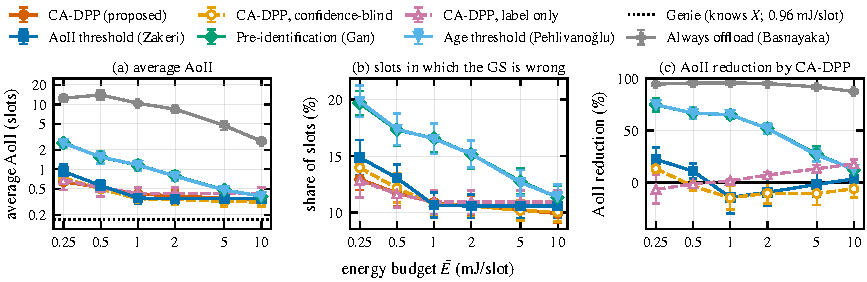
\includegraphics{figures/fig_budget.pdf}
\caption{Performance versus the energy budget $\bar E$: $20$ held-out runs per point ($5$-fold cross-validation over chips) with $95\%$ confidence intervals. (a) Average AoII. (b) Share of slots in which the GS is wrong. (c) AoII reduction of CA-DPP relative to each policy, with paired intervals (positive favors CA-DPP). CA-DPP beats the pre-identification, age-threshold and always-offload policies at every budget, and the AoII-threshold policy at $0.25$\,mJ/slot; from $1$\,mJ/slot on the two perform the same within statistical error. Baselines adapted from~\cite{zakeri2023aoiieh,gan2025taoi,pehlivanoglu2026orbit,basnayaka2025aomi}.}
\label{fig:budget}
\end{figure*}

Fig.~\ref{fig:budget} and Table~\ref{tab:results} compare CA-DPP with the baselines (Q2). Against the pre-identification and age-threshold policies, CA-DPP lowers the AoII by $75\%$ at $0.25$\,mJ/slot, $52\%$ at $2$\,mJ/slot and $12\%$ at $10$\,mJ/slot, in every fold up to $5$\,mJ/slot ($p<10^{-5}$). The pre-identification policy spends most of its energy on agreeing labels, which are worthless (Proposition~\ref{prop:confirm}). The age-threshold policy reacts to the time since the last delivery, which says little about whether the GS is wrong: an old status of a dry area that is still dry needs no update. Always offloading is an order of magnitude worse, since a raw frame costs $3$ to $21$ labels and often fails far from the GS.

Against the AoII-threshold policy, the outcome depends on the budget. At $0.25$\,mJ/slot, CA-DPP lowers the AoII by $22\%\pm12\%$ ($p=0.002$, four folds of five), and the $99$th percentile of the AoII drops from $19.2$ to $12.3$ slots. Here the UAV can send few labels, and the confidence decides which disagreements deserve them. At $0.5$\,mJ/slot the reduction is $11\%\pm7\%$ and not significant ($p=0.10$). From $1$\,mJ/slot on, the threshold policy with $k=1$ reports every disagreement for about $0.84$\,mJ/slot and matches CA-DPP; the differences range from $-3\%$ to $+14\%$ with $p\ge0.09$. When labels are this cheap, a wrong label is corrected within a slot or two, which the one-step gain of Lemma~\ref{lem:onestep} ignores; a discounted look-ahead did not help.


\subsection{Where the Gains Come From}\label{res:gains}
The two ablations answer Q2 and Q3 directly: the confidence-blind version removes the per-frame confidence, and the label-only version removes the raw uploads. At $0.25$\,mJ/slot the per-frame confidence matters: the confidence-blind version has a $15\%$ higher AoII ($p=0.001$). From $1$\,mJ/slot on, however, the confidence-blind version is $6\%$ to $15\%$ better than CA-DPP, and the difference is significant only at $1$\,mJ/slot ($p=0.02$). With this classifier, once energy is not scarce, the precision of each label value gives the belief most of what it needs. A plausible reason is that confident wrong labels come in runs, which the per-frame update over-counts.

Raw uploads pay off at larger budgets. Without them, the AoII stays at $0.43$ from $1$\,mJ/slot on, since the label-only version runs out of useful labels and spends only $0.65$\,mJ/slot. CA-DPP spends the rest on uploads and reaches $0.39$ at $2$\,mJ/slot and $0.34$ at $10$\,mJ/slot ($p\le0.001$). The genie reaches $0.171$ with $0.96$\,mJ/slot; the gap comes mostly from not seeing $X(t)$.

\emph{Mobility and the weight $V$.} CA-DPP exploits the trajectory although the distance enters~\eqref{eq:rule} only through $q_a(g)$ and $E_a(g)$. At $2$\,mJ/slot it uploads the frame in $5.9\%$ of the unblocked slots within $850$\,m of the GS and in $0.1\%$ beyond $2.15$\,km, where it sends labels instead ($2.0\%$ and $3.8\%$ of the slots). At $0.5$\,mJ/slot, raising $V$ from $10^{-3}$ to $3$ lowers the AoII from $0.79$ to $0.41$ but raises the energy spent over about $27{,}000$ slots from $0.50$ to $1.51$\,mJ/slot; values up to $10^{-2}$ stay within $4\%$ of the budget, so $V$ must match the mission length. A sample path and both sweeps are shown in Section~S3 of the supplementary material.

\subsection{Weak Classifiers, Blockage and Payload}\label{res:sens}
\begin{figure*}[t]
\centering
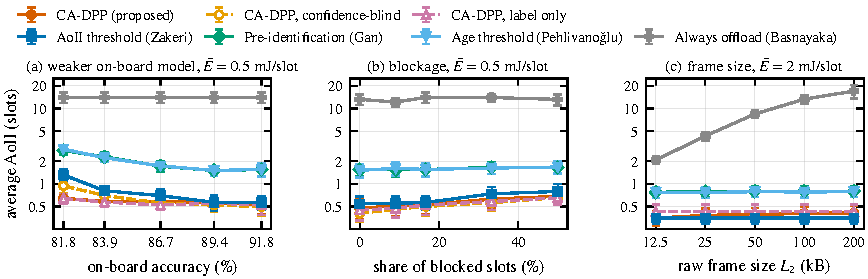
\includegraphics{figures/fig_sensitivity.pdf}
\caption{Sensitivity of the average AoII, $20$ held-out runs per point. (a) On-board accuracy (base model and four noisy variants) and (b) share of blocked slots $\rho_{\rm b}/(\rho_{\rm b}+\rho_{\rm u})$, both at $\bar E=0.5$\,mJ/slot. (c) Raw frame size $L_2$ at $\bar E=2$\,mJ/slot.}
\label{fig:sens}
\end{figure*}

In Fig.~\ref{fig:sens}(a), the AoII of CA-DPP grows only from $0.53$ to $0.64$ as the accuracy drops from $91.8\%$ to $81.8\%$. Over the same range, the AoII of the threshold policy grows from $0.56$ to $1.31$, and that of the confidence-blind version from $0.50$ to $0.94$. With the two noisiest models, it is $27\%$ and $49\%$ better than the threshold policy ($p<10^{-5}$) and $14\%$ and $28\%$ better than the confidence-blind version ($p\le0.003$), in all five folds. The noisiest model rarely says ``flooded'', so over a flooded area it mostly agrees with the wrong ``dry'' status of the GS. The threshold policy, which reacts only to disagreements, spends only $0.32$ of $0.5$\,mJ/slot. CA-DPP spends the full budget: a low-confidence ``dry'' frame barely lowers its belief that the GS is wrong, while a rare confident ``flooded'' frame raises it strongly, since flooded footprints are rare. The confidence-blind belief knows that ``dry'' labels are less reliable on average, but not which ones. Per-frame confidence pays off when the classifier is weak and its errors are lopsided, as is likely for a small model on a low-cost device.

As the share of blocked slots grows from $0$ to $50\%$ (Fig.~\ref{fig:sens}(b)), all policies lose ground and their order is unchanged. CA-DPP stays $9\%$ to $15\%$ below the threshold policy ($0.009\le p\le0.1$). The confidence-blind and label-only versions are $1.5\%$ to $11\%$ below CA-DPP at this budget, so at $0.5$\,mJ/slot raw uploads cost slightly more than they return. Fig.~\ref{fig:sens}(c) varies the size of the raw frame at $2$\,mJ/slot. With $12.5$\,kB frames, CA-DPP is $15\%$ better than the label-only version and matches the threshold policy. With $200$\,kB frames this advantage shrinks to $3.5\%$: uploads cost more and fail more often, and the policy uploads less without retuning.


\subsection{Optimality Gap, Correlated Errors and Robustness}\label{res:extra}
Section~S3 of the supplementary material reports four further checks; we summarize them here. \emph{Optimality gap.} A controller that also observes $X(t)$ can imitate any policy of (P), so its optimal AoII under the same budget, computed by value iteration on the Lagrangian with weak duality, lower-bounds the optimum of (P). In a synthetic model that satisfies Assumption~\ref{as:inf} (states from the fitted chain, classifier outputs resampled from data slots with the same state), CA-DPP with $\nu=1$ is within $14\%$ to $25\%$ of this bound from $0.25$ to $2$\,mJ/slot, and the AoII-threshold policy within $37\%$ to $71\%$. \emph{Correlated errors.} When the synthetic errors follow a Markov chain with persistence $\varrho$ (the traces have $\varrho=0.56$), the advantage of CA-DPP over the threshold policy at $2$\,mJ/slot falls from $23\%$ with independent errors to about $1\%$ at the persistence of the traces with $\nu=1$; the correlation rule for $\nu$ recovers part of it, and at $0.5$\,mJ/slot CA-DPP stays $20\%$ to $34\%$ ahead at every persistence. This points to correlated errors as the cause of the tie at large budgets on the real traces. \emph{Robustness.} With $\nu$ from the correlation rule instead of tuning, CA-DPP beats the threshold policy by $11\%$ to $16\%$ at $0.5$, $5$ and $10$\,mJ/slot but only ties at $0.25$\,mJ/slot, so choosing $\nu$ per budget is the safer default. With the exact fading-averaged energy instead of~\eqref{eq:energy}, the AoII of CA-DPP changes by at most $6.7\%$ and no significant comparison changes sign. A belief-threshold rule that sends a label when $\mu_t$ exceeds a tuned threshold performs as well as CA-DPP (paired $p\ge0.10$), so the belief carries most of the gain over the AoII-threshold policy; CA-DPP adds budget control with the guarantee of Theorem~\ref{thm:budget} and per-slot adaptation to the link. \emph{Statistics.} Tested on the five fold means rather than the $20$ runs, the gains with the two weakest classifiers remain significant ($p=0.035$ and $p=0.014$), whereas the $0.25$\,mJ/slot gain, seen in four of five folds, has $p=0.17$.

%% =====================================================================
\section{Discussion}\label{sec:discussion}
%% =====================================================================
\subsection{Answers to the Research Questions}
\emph{Q1.} Never send an agreeing label; otherwise take the action whose value $q_a(g)G_a$ most exceeds its priced energy, which gives confidence thresholds ordered silent, raw upload, label (Proposition~\ref{prop:threshold}), and the price keeps the budget (Theorem~\ref{thm:budget}).

\emph{Q2.} The per-frame confidence helps when updates are scarce, either because energy is scarce or because the classifier is weak. The UAV must then choose which few disagreements to report, and the confidence ranks them. When energy is ample and the classifier accurate, every disagreement can be reported and a simple rule does as well.

\emph{Q3.} The value of raw uploads depends on the link more than on the classifier. Uploads pay off at budgets of $2$\,mJ/slot and above, near the GS and with small frames.

Two design lessons follow. First, never send a label that agrees with the receiver (Proposition~\ref{prop:confirm}); much of the $52\%$ to $75\%$ gap to the pre-identification and age-threshold policies comes from the energy they spend on such labels. Second, calibrate the classifier on board: isotonic calibration is a lookup table, and the prior correction~\eqref{eq:lik} matters because monitored events are rare.

\subsection{Correlated Errors}
The main weakness of CA-DPP at large budgets is Assumption~\ref{as:inf}(ii): the on-board errors come in runs (Section~\ref{res:cls}). The tempered update~\eqref{eq:post} discounts every frame equally and cannot tell new evidence from a repeated error. Section~\ref{res:extra} shows that this costs CA-DPP most of its advantage over the threshold policy at large budgets, and that the rule for $\nu$ recovers part of it. A hidden Markov model of the classifier state could recover more, at twice the belief size.

\subsection{Other IoT Settings}
Nothing in the model is specific to UAVs or floods. The link and energy models fit any device whose channel varies predictably, such as a low-Earth-orbit satellite that sees a ground station only during passes. A non-binary scene needs a belief over the AoII and the current class, but the gains keep their structure: a right update removes AoII and a wrong one creates it.

\subsection{Limitations}
Five limitations remain. First, the policy is myopic; its gap to the optimal policy of (P) is bounded only numerically, in a model with independent errors (Section~\ref{res:extra}). Second, Proposition~\ref{prop:threshold} holds for the per-slot rule~\eqref{eq:rule} within each confidence bin; whether the optimal policy of (P) shares it is open. Third, Sentinel-2 imagery stands in for UAV frames (FLAME~\cite{shamsoshoara2021flame} and AIDER~\cite{kyrkou2020aider} are UAV alternatives). Fourth, the energy model is analytic; replacing the mean-SNR approximation~\eqref{eq:energy} by the exact fading average changes none of the conclusions (Section~\ref{res:extra}), but measured energy is still missing. Fifth, the imagery is not tied to the UAV position, so route planning is left out.

%% =====================================================================
\section{Conclusion}\label{sec:concl}
%% =====================================================================
We studied status updates from an IoT device whose sensor is its own classifier, with a UAV mapping a flood as the running example. A belief over the AoII of the GS status, updated with the calibrated confidence of each frame, gives closed-form values of the three actions: agreeing labels are worthless, and the per-slot decision has confidence thresholds ordered silent, raw, label. CA-DPP, built on them, meets the energy budget on every sample path. On flood-mapping traces under chip-level cross-validation, it beats adaptations of three recent designs at every budget up to $5$\,mJ per slot, and an AoII-threshold policy when energy is scarce or the classifier is weak. Raw uploads pay off near the GS at larger budgets. Next steps are a belief that models correlated errors, and UAV imagery with measured energy.

\ifCLASSOPTIONcompsoc
  \section*{Acknowledgments}
\else
  \section*{Acknowledgment}
\fi
No specific grant from any funding agency in the public, commercial or not-for-profit sectors supported this work. The author declares no competing interests. The Sen1Floods11 dataset~\cite{bonafilia2020sen1floods11} is publicly available, and the simulation code, inference traces and scripts that produce every figure and table are available at \url{https://github.com/sshawky78AUA/confidence-aware-status-update-IoT}. In line with the IEEE policy on AI-generated content, the author discloses that Claude (Anthropic) was used to assist with drafting and editing the text of all sections, writing the simulation and plotting code, and preparing the figures. The author reviewed and edited all such content and takes full responsibility for the article.

\bibliographystyle{IEEEtran}
\bibliography{refs}

%% Author biography and photo are kept out of this public copy (see the Overleaf project or the project files).

\end{document}
